\section{Problem Definition}\label{sec:problem}

\begin{figure}[t]
    \centering
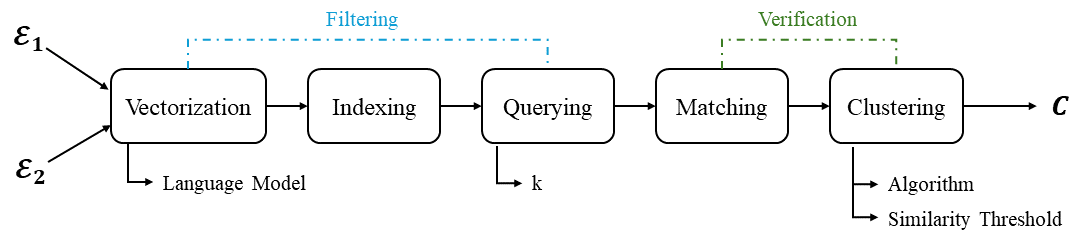
\includegraphics[width=0.97\linewidth]{figures/pyjedai/pipeline-AutoER.png}
    % \vspace{-20pt}
    \caption{The ETEER pipeline considered in this work.}
    \label{fig:eeter_pipeline}
    % \vspace{-12pt}
\end{figure}

%In this section, we describe the problem that this paper tackles, which is end-to-end entity resolution, namely ETEER. We define two variations of this problem, depending on whether ground truth knowledge is available or not. 

Let an \emph{entity collection} $\mathcal{E}$ be a set of entity descriptions, where each description (also called ``entity'' for brevity)
%, we will also refer to entity descriptions, simply as .} 
is a set of attribute-value pairs representing a real-world entity (e.g., an entity description can be a database record, a row in a csv file, a json element or an ontology class instance). 

End-to-end ER (ETEER) is the problem of receiving one or more entity collections and returning a set of entity \emph{clusters}, with each cluster corresponding to a set of entity descriptions that refer to the same real-world entity. 
%Although ER can be generalized to receive as input one (Dirty ER~\cite{DBLP:journals/pvldb/HassanzadehCML09}), two (Clean-Clean ER~\cite{DBLP:journals/vldb/PapadakisETHC23}), or more than two (Multi-Source ER~\cite{DBLP:conf/esws/SaeediPR20,DBLP:conf/adbis/SaeediPR17}) entity collections, in this work, we will assume the case of two clean (i.e., duplicate-free) entity collections $\mathcal{E}_1$ and $\mathcal{E}_2$ that need to be resolved. Our definitions and methodology can be easily generalized to cover all other cases. 

More formally:
% \begin{problem} 
% \label{pr:eteer}
% Given two entity collections $\mathcal{E}_1$ and $\mathcal{E}_2$, cluster them into a set of disjoint clusters $\mathcal{C}$, such that $\forall c_i, c_j \in \mathcal{C}\;  c_i \cap c_j = \emptyset$, with $i \neq j$, 
% and $c_i \subset \mathcal{E}_1 \cap \mathcal{E}_2$, if $|c_i|=2$, or $c_i \subset \mathcal{E}_1 \cup \mathcal{E}_2$, if  $|c_i|=1$.
% \end{problem}
\vspace{4pt}
\begin{definition}[End-to-end Entity Resolution (ETEER)]\label{def:eteer}
Given two entity collections $\mathcal{E}_1$ and $\mathcal{E}_2$, return a set of disjoint clusters $\mathcal{C}$, such that 
$\bigcup_{c_l \in \mathcal{C}}c_l = \mathcal{E}_1 \cup \mathcal{E}_2$, and
$\forall c_l \in \mathcal{C}, 
 e_i \in \mathcal{E}_1 \cap c_l, e_j \in \mathcal{E}_2 \cap c_l \Rightarrow e_i \equiv e_j$, 
where $e_i \equiv e_j$ denotes that the two entity descriptions~\emph{match} {(i.e., they correspond to identical real-world objects)}.
%, referring to the same real-world entity.
\end{definition}
\vspace{4pt}

% \begin{problem} 
% \label{pr:eteer_alternative}
% \comments{[alternative def]}
% Given two entity collections $\mathcal{E}_1$ and $\mathcal{E}_2$, cluster them into a set of disjoint clusters $\mathcal{C}$, such that 
% $\bigcup_{c_i \in \mathcal{C}}c_i = \mathcal{C}$, and
% $\forall c_i \in \mathcal{C}, 
% |c_i|=2$, if $c_i \subseteq \mathcal{E}_1 \cap \mathcal{E}_2$, otherwise, $|c_i|=1$. 
% \end{problem}

This definition applies to Record Linkage \cite{DBLP:books/daglib/0030287}, also known as Clean-Clean ER~\cite{DBLP:journals/vldb/PapadakisETHC23}, where $\mathcal{E}_1$ and $\mathcal{E}_2$ are individually duplicate-free, but overlapping, sharing some entities. In this setting, each cluster contains either a single  entity from one entity collection, or 
%two entities,
one from each collection. Definition~\ref{def:eteer} can be easily generalized to Dirty ER \cite{DBLP:journals/pvldb/HassanzadehCML09}, also known as Deduplication \cite{DBLP:books/daglib/0030287}, where the input comprises a single entity collection with duplicates in itself. In this case, the resulting clusters are also disjoint, but there is no limit on their size, i.e., the number of entities they contain. It can also be generalized to the case of Multi-Source ER \cite{DBLP:conf/esws/SaeediPR20,DBLP:conf/adbis/SaeediPR17}, where the input comprises multiple, duplicate-free entity collections. This setting requires that each cluster cannot contain more than one entity from the same collection. 

% The problem of Definition~\ref{def:eteer} is typically solved through an ETEER pipeline, denoted by $w(\mathcal{E}_1, \mathcal{E}_2)$, whose \underline{effectiveness} is assessed with respect to: i) \textit{Precision}, which is is the portion of pairs in $\mathcal{C}$ that are indeed matching, ii) \textit{Recall}, which is is the portion of pairs in $\mathcal{D}$ that co-occur in some cluster of $\mathcal{C}$, where $\mathcal{D}$ denotes the set of duplicate entities, and iii) \textit{F-Measure}, which is the harmonic mean of Precision and Recall. The \underline{time efficiency} of $w(\mathcal{E}_1, \mathcal{E}_2)$ is measured in terms of the overall run-time, i.e., the time intervenes between receiving $\mathcal{E}_1$ and $\mathcal{E}_2$ and producing $\mathcal{C}$.

The problem of Definition~\ref{def:eteer} is typically solved through an \emph{ETEER pipeline}, also called \emph{workflow}, denoted by $w(\mathcal{E}_1, \mathcal{E}_2)$. This involves a series of processing steps, which potentially require the configuration of some parameters. More formally:
\vspace{4pt}
\begin{definition}[ETEER Pipeline]
An ETEER Pipeline $w(\mathcal{E}_1, \mathcal{E}_2) = (S, P, V)$ is a series of processing steps $S = s_1, s_2, \ldots, s_n$ for solving ETEER, with each processing step $s_i$ potentially requiring the configuration of some parameters $P_i = p_1^i, p_2^i, \ldots, p_m^i$, and with each parameter $p_j^i$ accepting a set of possible values $V_j^i$.
\end{definition}
\vspace{4pt}

Following the previous definition, we 
%will sometimes simply 
call the set $P = \bigcup\limits_{i \in [1..n]}
P_i$ \emph{configuration parameters} and 
%we will also simply call 
the set $V = \bigcup\limits_{P_i \in P, p_j \in P_i}V_j^i$ as \emph{configuration values} or \emph{possible values}.

The \underline{effectiveness} of an ETEER pipeline is assessed in terms of precision, recall, and F1-score, with respect to the ground truth of known matches $\mathcal{D}$. In more detail,
\textit{precision} is the portion of clusters in $\mathcal{C}$ which contain a pair of entities that also appears in $\mathcal{D}$; 
\textit{recall} is the portion of pairs in $\mathcal{D}$ that co-occur in some cluster of $\mathcal{C}$;
\textit{F1-score} is the harmonic mean of precision and recall.

The \underline{time efficiency} of an ETEER pipeline can be measured in terms of the 
overall runtime, i.e., the time between receiving $\mathcal{E}_1$ and $\mathcal{E}_2$ and producing $\mathcal{C}$. 
%Given that we are interested in finding the best configuration for a fixed ETEER pipeline, we will focus more on measuring time efficiency of AutoER in terms 
In this work, we also consider
%Another crucial aspect is
the \emph{search time}, i.e., the time needed to %produce a the suggested 
recommend configuration values.


In this context, we address two problems for fine-tuning ETEER pipelines, based on whether a ground truth is available (Problem~\ref{pr:pr1}) or not (Problem~\ref{pr:pr2}).
%for configuration tuning. 
%Such a (subset of the) ground truth is also known as ``seed alignment'' and is used for training entity alignment models~\cite{DBLP:journals/datamine/FanourakisEKC23,DBLP:journals/pvldb/SunZHWCAL20}. 
For the evaluation, we always use the ground truth of known matches $\mathcal{D}$. In Problem~\ref{pr:pr1}, we also use $\mathcal{D}$
%a portion of the ground truth 
for tuning the configuration parameters, unlike Problem~\ref{pr:pr2}.
More formally:
%, we do not use any portion of the ground truth.

% $\bullet$ \textit{Specified ETEER pipeline and ground truth.} The goal is to fine-tune a specific ETEER pipeline provided that some subset of the golden standard of real matches is available. This task can be formalized as follows:
% \Figure[t!](topskip=0pt, botskip=0pt, midskip=0pt, wid){figures/pyjedai/pipeline-AutoER.png}
% {The ETEER pipeline considered in this work.}
\vspace{4pt}
\begin{problem}\label{pr:pr1}
Given an ETEER pipeline $w(\mathcal{E}_1, \mathcal{E}_2)$ for two entity collections $\mathcal{E}_1$ and $\mathcal{E}_2$, along with a subset of the ground truth of matches $\mathcal{D}' \subseteq \mathcal{D}$, return the configuration values $V' \subseteq V$ of $w(\mathcal{E}_1, \mathcal{E}_2)$ that maximize the effectiveness of $w(\mathcal{E}_1, \mathcal{E}_2)$ in terms of F1-score, while minimizing the search time.
\end{problem}
\vspace{4pt}
For the returned configuration values $V'$, it holds that $|V'| = |P|$, i.e., one value should be returned for each configuration parameter.

The na\"ive approach is to apply \textit{grid search}, considering all meaningful values for all configuration parameters in the specified pipeline. However, this is impractical and time-consuming, due to the enormous configuration space.
%even for simple ETEER pipelines, because they typically involve numerous configuration parameters with large domains. Therefore, 
More advanced algorithms for configuration optimization are required to effectively restrict the search to a small portion of the configuration space.
%extremely large search space of configuration parameters. 

% $\bullet$ \textit{Specified ETEER pipeline without ground truth.} 

A more difficult variation of the first problem is to fine-tune a specific ETEER pipeline without having any portion of the real matches $\mathcal{D}$ provided as input. This task can be formalized as follows:

\vspace{4pt}
\begin{problem}
\label{pr:pr2}
Given an ETEER pipeline $w(\mathcal{E}_1, \mathcal{E}_2)$ for two entity collections $\mathcal{E}_1$ and $\mathcal{E}_2$, {without relying on their ground truth}, return the configuration values $V' \subseteq V$ of $w(\mathcal{E}_1, \mathcal{E}_2)$ that maximize the effectiveness of $w(\mathcal{E}_1, \mathcal{E}_2)$ in terms of F1-score, while minimizing the search time.
% Given an ETEER pipeline $w(\mathcal{E}_1, \mathcal{E}_2)$ and two entity collections, $\mathcal{E}_1$ and $\mathcal{E}_2$, optimize the configuration parameters of $w(\mathcal{E}_1, \mathcal{E}_2)$ so as to maximize its effectiveness in terms of F-Measure, while minimizing the search time.
\end{problem}
\vspace{4pt}

To the best of our knowledge, no prior work on ER examines these tasks, even though both can be solved by existing techniques. 